\documentclass{article}

\usepackage{graphicx}
\usepackage{tikz}
\usepackage{tikzsymbols}
\usetikzlibrary{calc,patterns,shapes.geometric}
\pagestyle{empty}
\usepackage[margin=0pt]{geometry}
\geometry{papersize={14in,12in}}

\def\centerarc[#1](#2)(#3:#4:#5){\draw[#1] ($(#2)+({#5*cos(#3)},{#5*sin(#3)})$) arc (#3:#4:#5);}

\begin{document}
	\begin{figure}
		\centering
		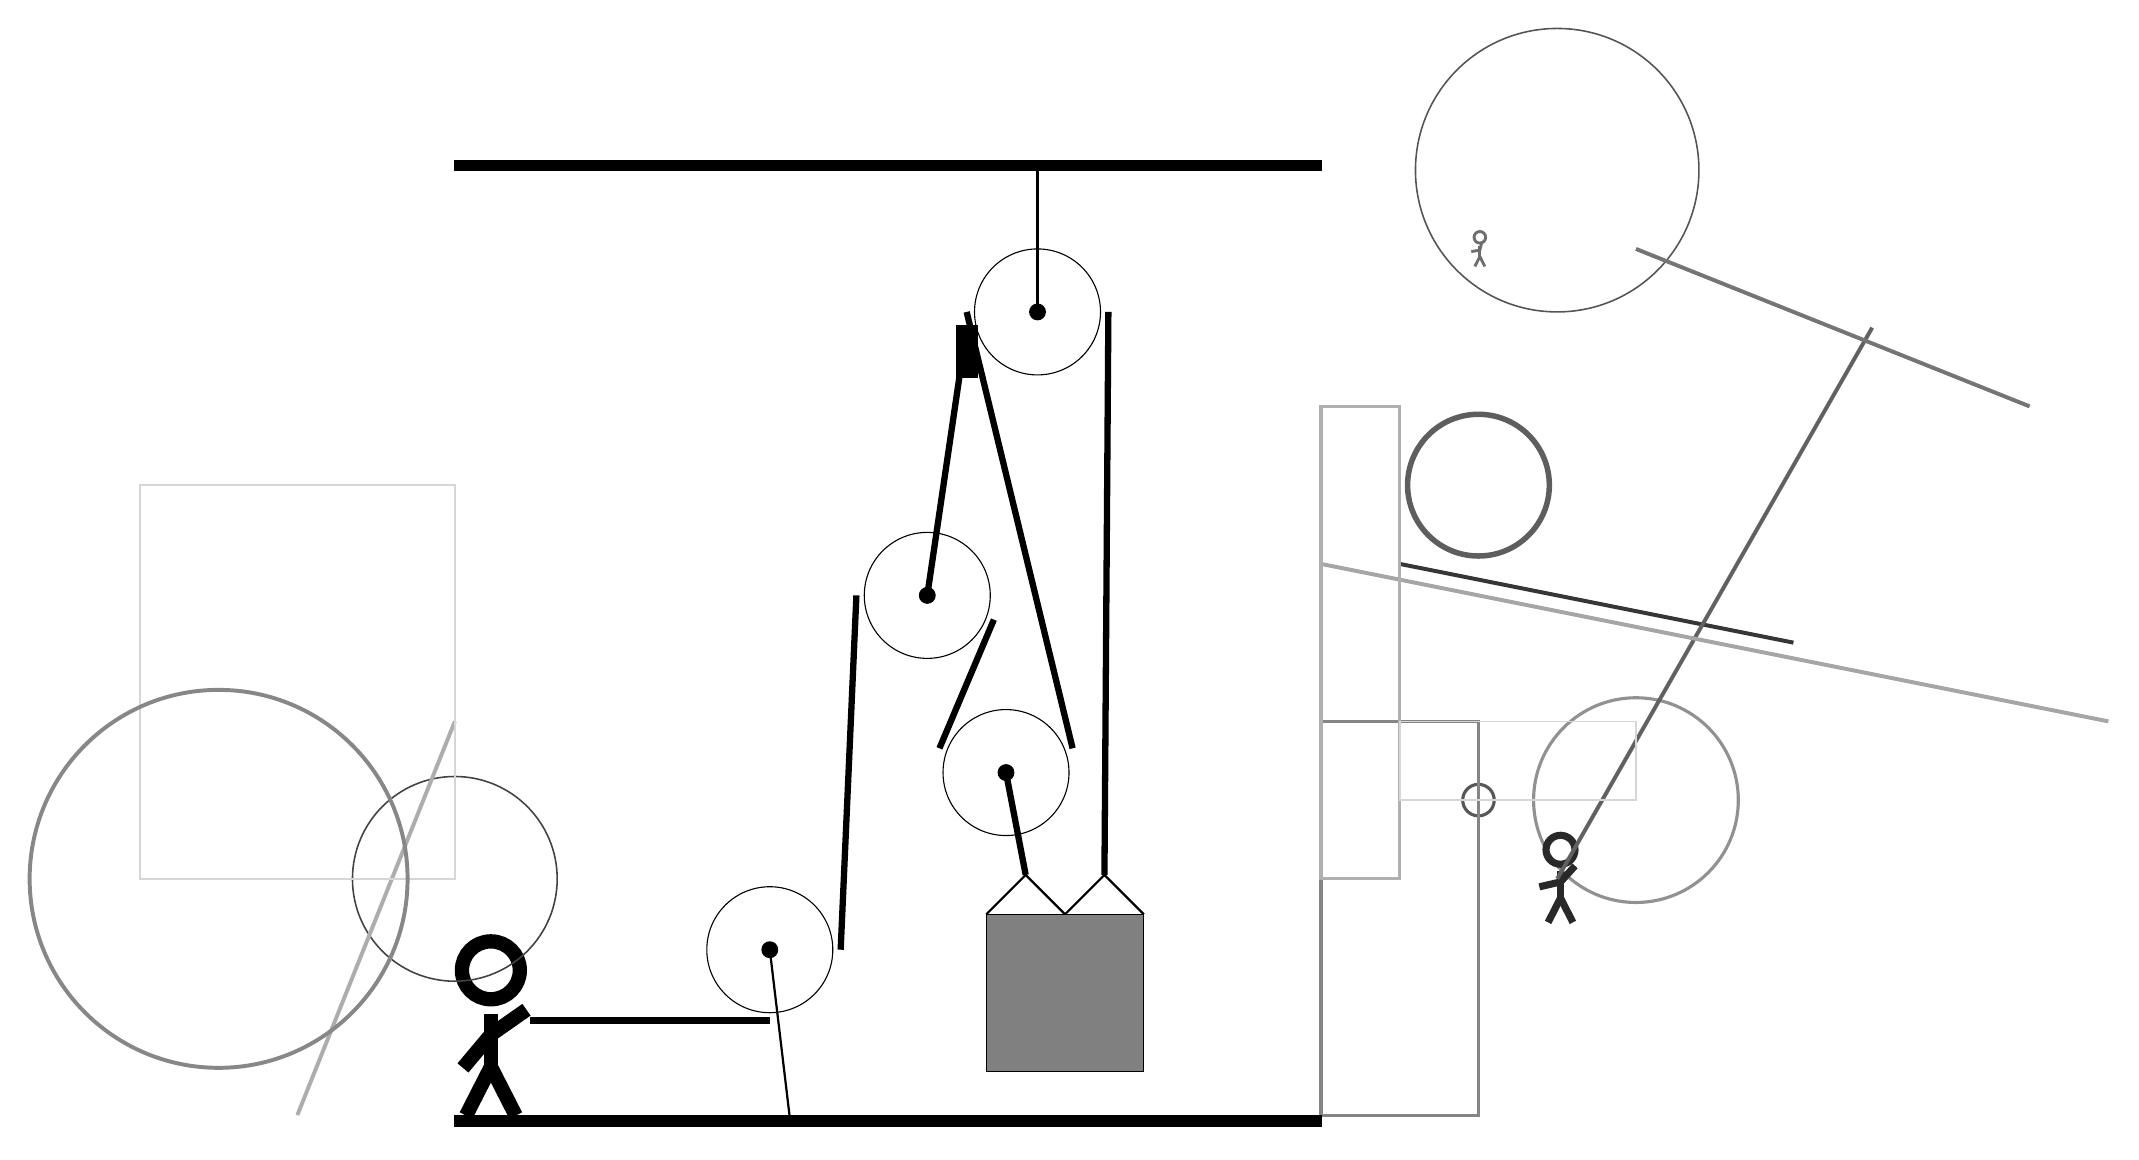
\begin{tikzpicture}
			%%%%% START %%%%%
			
			\draw[fill=black] (-6, 9) rectangle (5, 9.125);
			
			\draw (0, 3.6) circle (0.8);
			\draw[fill=black] (0, 3.6) circle (0.1);
			
			\draw (1, 1.35) circle (0.8);
			\draw[fill=black] (1, 1.35) circle (0.1);
			
			\draw (1.4, 7.2) circle (0.8);
			\draw[fill=black] (1.4, 7.2) circle (0.1);
			\draw[very thick] (1.4, 7.2) -- (1.4, 9);
			
			\draw (-2, -0.9) circle (0.8);
			\draw[fill=black] (-2, -0.9) circle (0.1);
			\draw[thick] (-2, -0.9) -- (-1.75, -3);
			
			
			\draw[thick]  (0.75, -0.45) -- (1.25, 0.05) -- (1.75, -0.45) -- (2.25, 0.05) -- (2.75, -0.45);
			\draw[fill=black!50] (0.75, -0.45) rectangle (2.75, -2.45);
			\draw[line width=0.8mm] (-5.05, -1.8) -- (-2, -1.8);
			\centerarc[line width=0.8mm](-2, -0.9)(270:360:0.9);
			\draw[line width=0.8mm] (-1.1, -0.9) -- (-0.9, 3.6);
			\draw[line width=0.8mm] (0, 3.6) -- (0.5, 7.0);
			\draw[line width=0.8mm, fill=black](0.4, 6.4) rectangle (0.6, 7.0);
			\centerarc[line width=0.8mm](0, 3.6)(-20:180:0.9);
			\draw[line width=0.8mm] (0.8457, 3.2922) -- (0.1543, 1.6578);
			\centerarc[line width=0.8mm](1, 1.35)(160:380:0.9);
			\draw[line width=0.8mm] (1.8457, 1.6578) -- (0.5, 7.2);
			\draw[line width=0.8mm](1, 1.35) -- (1.25, 0.05);
			\centerarc[line width=0.8mm](1.4, 7.2)(0:180:0.9);
			\draw[line width=0.8mm] (2.3, 7.2) -- (2.25, 0.05);
			
			\node at (-5.5, -1.9) {\Strichmaxerl[10][50][35]};
			
			\draw [line width=0.2mm, color=black!74](-6, 0) circle (1.3);
			
			\draw[line width=0.5mm, color=black!32](-8, -3) -- (-6, 2);
			\draw [line width=0.4mm, color=black!43](9, 1) circle (1.3);
			\draw[line width=0.3mm, color=black!16] (-6, 0) rectangle (-10, 5);
			
			\draw [line width=0.4mm, color=black!66](7, 1) circle (0.2);
			\draw[line width=0.5mm, color=black!79](6, 4) -- (11, 3);
			\draw [line width=0.5mm, color=black!47](-9, 0) circle (2.4);
			
			\node[line width=0.7mm, color=black!84] at (8, 0) {\Strichmaxerl[5][13][48]};
			\draw[line width=0.4mm, color=black!28] (6, 6) rectangle (6, 2);
			\draw[line width=0.2mm, color=black!74] (7, 2) rectangle (6, 1);
			
			\draw[line width=0.4mm, color=black!48] (5, 2) rectangle (7, -3);
			
			\draw[line width=0.5mm, color=black!62](8, 0) -- (12, 7);
			\draw[line width=0.5mm, color=black!35](5, 4) -- (15, 2);
			\node[line width=0.2mm, color=black!57] at (7, 8) {\Strichmaxerl[2][9][76]};
			\draw [line width=0.2mm, color=black!67](8, 9) circle (1.8);
			\draw[line width=0.4mm, color=black!31] (6, 6) rectangle (5, 0);
			
			\draw[line width=0.2mm, color=black!16] (6, 1) rectangle (9, 2);
			\draw [line width=0.7mm, color=black!63](7, 5) circle (0.9);
			\draw[line width=0.5mm, color=black!54](9, 8) -- (14, 6);
			
			
			\draw[fill=black] (-6, -3) rectangle (5, -3.15);
			
			%%%%% END %%%%%
		\end{tikzpicture}
	\end{figure}	
\end{document}